\documentclass{beamer}
\usepackage{pdfpages}
%Imports and customization
\usepackage{tikz}
\usepackage{graphicx}
\usepackage{tikz-feynman}
\usepackage{ulem}
\usepackage{colortbl}
\graphicspath{ 
    {./images/}
}

\beamertemplatenavigationsymbolsempty
\setbeamertemplate{sidebar right}{}
\setbeamertemplate{footline}{
    \hfill\usebeamertemplate***{navigation symbols}
    \hspace{1cm}\insertframenumber{}/\inserttotalframenumber
}
\setbeamertemplate{caption}{\raggedright\insertcaption\par}
\setbeamersize{text margin left=4mm,text margin right=4mm} 

\setbeamerfont{itemize/enumerate body}{size=\scriptsize}
\setbeamerfont{itemize/enumerate subbody}{size=\scriptsize}
\setbeamerfont{itemize/enumerate subsubbody}{size=\scriptsize}


%Custom Macros
\newcommand{\statwarn}{
    \tiny \color{red} Absolute numbers here mean NOTHING. Plots are based on small (100k events) samples, and are highly biased. All that matters is relative position!
}


% WARNING: When using these commands, the image argument must
% NOT have spaces between itself and the braces
\newcommand{\fullscreenimage}[2]{
    \frame{
        \frametitle{#1} 
        \begin{figure}
        \includegraphics[height=0.9\textheight,width=\textwidth,keepaspectratio]{#2}
        \end{figure}
    }
}


\newcommand{\importpdf}[3]{
    \frame{
        \begin{columns}\column{\dimexpr\paperwidth-10pt}
        \begin{figure}
        \includegraphics[page=#2,height=0.8\textheight,width=\textwidth,keepaspectratio]{#1}
        \end{figure}

        {\tiny #3}
        \end{columns}
    }
}


\newcommand{\displayone}[3]{
    \frame{
        \frametitle{#1} 
        \begin{columns}
            \begin{column}{0.5\textwidth}
                #2
            \end{column}
            \begin{column}{0.5\textwidth}
                \begin{figure}
                    \includegraphics[width=\linewidth,height=\textheight,keepaspectratio]{#3}
                \end{figure}
            \end{column}
        \end{columns}
    }
}

\newcommand{\displayonelarge}[3]{
    \frame{
        \frametitle{#1} 
        \begin{columns}
            \begin{column}{0.3\textwidth}
                #2
            \end{column}
            \begin{column}{0.7\textwidth}
                \begin{figure}
                    \includegraphics[width=\linewidth,height=0.8\textheight,keepaspectratio]{#3}
                \end{figure}
            \end{column}
        \end{columns}
    }
}


\newcommand{\displaytwo}[4]{
    \frame{
        \frametitle{#1} 
        #2
        \begin{columns}
            \begin{column}{0.5\textwidth}
                \begin{figure}
                    \includegraphics[width=\linewidth,height=\textheight,keepaspectratio]{#3}
                \end{figure}
            \end{column}
            \begin{column}{0.5\textwidth}
                \begin{figure}
                    \includegraphics[width=\linewidth,height=\textheight,keepaspectratio]{#4}
                \end{figure}
            \end{column}
        \end{columns}
    }
}

\newcommand{\displaytwocaption}[6]{
    \frame{
        \frametitle{#1} 
        #2
        \begin{columns}
            \begin{column}{0.5\textwidth}
                \begin{figure}
                    \includegraphics[width=\linewidth,height=\textheight,keepaspectratio]{#3}
                    \caption{#4}
                \end{figure}
            \end{column}
            \begin{column}{0.5\textwidth}
                \begin{figure}
                    \includegraphics[width=\linewidth,height=\textheight,keepaspectratio]{#5}
                    \caption{#6}
                \end{figure}
            \end{column}
        \end{columns}
    }
}

\newcommand{\displaytwoVcaption}[6]{
    \frame{
        \begin{columns}
            \begin{column}{0.5\textwidth}
                \frametitle{#1} 
                #2
            \end{column}
            \begin{column}{0.5\textwidth}
                \begin{figure}
                    \includegraphics[width=\linewidth,height=0.3\textheight,keepaspectratio]{#3}
                    \caption{#4}
                \end{figure}

                \begin{figure}
                    \includegraphics[width=\linewidth,height=0.3\textheight,keepaspectratio]{#5}
                    \caption{#6}
                \end{figure}
            \end{column}
        \end{columns}
    }
}


\newcommand{\displaythree}[5]{
    \frame{
        \begin{columns}[T]
            \begin{column}{0.4\textwidth}
                {\usebeamercolor[fg]{title} \insertframetitle{#1} }\\
                \vspace{5mm}
                #2
            \end{column}
            \begin{column}{0.4\textwidth}
                \begin{figure}
                    \includegraphics[width=\linewidth,height=\textheight,keepaspectratio]{#3}
                \end{figure}
            \end{column}
        \end{columns}
        \begin{columns}[T]
            \begin{column}{0.4\textwidth}
                \begin{figure}
                    \includegraphics[width=\linewidth,height=\textheight,keepaspectratio]{#4}
                \end{figure}
            \end{column}
            \begin{column}{0.4\textwidth}
                \begin{figure}
                    \includegraphics[width=\linewidth,height=\textheight,keepaspectratio]{#5}
                \end{figure}
            \end{column}
        \end{columns}
    }
}


\newcommand{\displayfour}[5]{
    \frame{
        \frametitle{#1} 
        \begin{columns}[T]
            \begin{column}{0.4\textwidth}
                \begin{figure}
                    \includegraphics[width=\linewidth,height=\textheight,keepaspectratio]{#2}
                \end{figure}
            \end{column}
            \begin{column}{0.4\textwidth}
                \begin{figure}
                    \includegraphics[width=\linewidth,height=\textheight,keepaspectratio]{#3}
                \end{figure}
            \end{column}
        \end{columns}
        \begin{columns}[T]
            \begin{column}{0.4\textwidth}
                \begin{figure}
                    \includegraphics[width=\linewidth,height=\textheight,keepaspectratio]{#4}
                \end{figure}
            \end{column}
            \begin{column}{0.4\textwidth}
                \begin{figure}
                    \includegraphics[width=\linewidth,height=\textheight,keepaspectratio]{#5}
                \end{figure}
            \end{column}
        \end{columns}
    }
}


\newcommand{\pstrike}[2]{
    \only<-\the\numexpr#1-1>{#2}
    \only<#1->{\sout{#2}}
}


\newcommand{\announcesection}[1]{
    \section{#1}
    \frame{
        \begin{center}
            {\huge #1} 
        \end{center}
    }
}

\newcommand{\kvv}{\kappa_{2V}}
\newcommand{\kl}{\kappa_{\lambda}}
\newcommand{\kv}{\kappa_{V}}

\newcommand{\fkvv}[1]{\kappa_{2V,#1}}
\newcommand{\fkl} [1]{\kappa_{\lambda,#1}}
\newcommand{\fkv} [1]{\kappa_{V,#1}}

\newcommand{\importpdfwpages}[3]{
    \foreach \pageN in {#2,...,#3}{
        \importpdf{#1}{\pageN}{}
    }
}

\newcommand{\hyper}[2]{{\color{blue}\href{#1}{#2}}}



%Begin Presentation
\begin{document}
    \setbeamercolor{background canvas}{bg=}
    \title{VBF Signals Combinations and Re-Weightings}
    \author{Chris Milke}
    \date{07 January, 2021}

    \frame{\titlepage}
    %\frame{\frametitle{Overview} \tableofcontents}

    \section{Linear Algebra}

% show diagrams with terms, then show squaring
\frame{
    \frametitle{3D Coupling Dependence}
    \begin{figure}
    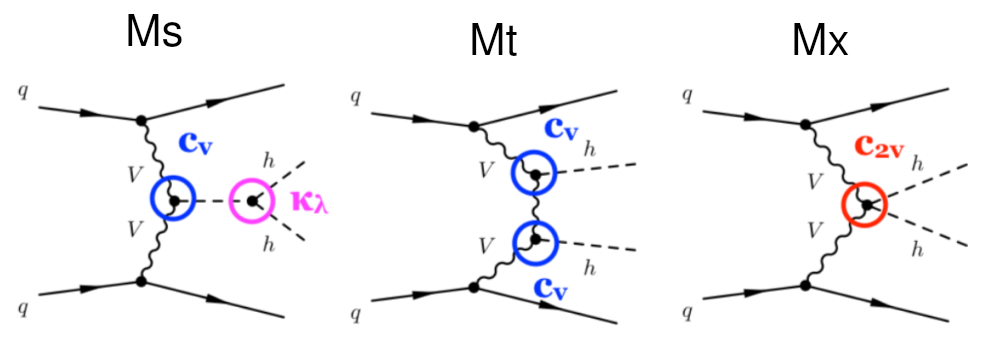
\includegraphics[width=0.6\linewidth,height=0.6\textheight,keepaspectratio]{vbf-hh_diagrams2b}
    \end{figure}
    $ \sigma = | \kv \kl M_s + \kv^2 M_t + \kvv M_x |^2 = $

    \vspace{10mm}

    $ \kv^2 \kl^2 M_s^2 + \kv^4 M_t^2 + \kvv^2 M_x^2 
    + \kv^3 \kl (M_s^* M_t + M_t^* M_s) 
    + \kv \kl \kvv (M_s^* M_x + M_x^* M_s ) 
    + \kv^2 \kvv (M_t^* M_x + M_x^* M_t )$

    \vspace{10mm}

    $ \sigma = \kv^2 \kl^2 a_1 + \kv^4 a_2 + \kvv^2 a_3 + \kv^3 \kl a_4 + \kv \kl \kvv a_5 + \kv^2 \kvv a_6 $
}

% convert to matrix, show nice matrix solution
\frame{
    \frametitle{Reweighting Solved via Linear Algebra}

    \begin{columns}[T]
        \begin{column}{0.18\textwidth}
            $ \vec{\sigma} = \begin{pmatrix} \sigma_1 \\
                \sigma_2 \\ \sigma_3 \\ \sigma_4 \\
                \sigma_5 \\ \sigma_6 \end{pmatrix} $
        \end{column}
        \begin{column}{0.15\textwidth}
            $ \vec{a} = \begin{pmatrix} a_1 \\ a_2 \\ a_3 \\ a_4 \\ a_5 \\ a_6 \end{pmatrix} $
        \end{column}
        \begin{column}{0.25\textwidth}
            $ \vec{f} = \begin{pmatrix} \kv^2 \kl^2 \\ \kv^4 \\ \kvv^2 \\ \kv^3 \kl \\ \kv \kl \kvv \\ \kv^2 \kvv \end{pmatrix} $
        \end{column}
        \begin{column}{0.4\textwidth}
            $ F = \begin{pmatrix}
                \vec{f}(\fkvv{1}, \fkl{1}, \fkv{1}) \\
                \vec{f}(\fkvv{2}, \fkl{2}, \fkv{2}) \\
                \vec{f}(\fkvv{3}, \fkl{3}, \fkv{3}) \\
                \vec{f}(\fkvv{4}, \fkl{4}, \fkv{4}) \\
                \vec{f}(\fkvv{5}, \fkl{5}, \fkv{5}) \\
                \vec{f}(\fkvv{6}, \fkl{6}, \fkv{6}) \\
            \end{pmatrix} $
        \end{column}
    \end{columns}

    \vspace{10mm}

    $ \vec{\sigma} = F \bullet \vec{a} \; \Longrightarrow \; \vec{a} = F^{-1} \bullet \vec{\sigma} $

    \vspace{10mm}

    $ \boxed{ \sigma(\kvv,\kl,\kv) = \vec{f}(\kvv,\kl,\kv) \bullet F^{-1} \bullet \vec{\sigma} } $
}

    \section{Orthogonal Basis States}

\frame{
    \frametitle{Initial Attempt at a Basis Set}
    \begin{columns}
        \begin{column}{0.4\textwidth}
            \begin{center} 
            Basis Set
            \resizebox{0.4\textheight}{!}{\begin{tabular}{ |l|l|l| }
                \hline
                \textbf {$\kappa_{2V}$} & \textbf {$\kappa_\lambda$} & \textbf {$\kappa_V$} \\
                \hline
                1   &  1 &   1 \\
                1   &  0 &  -1 \\
                0   &  1 &   1 \\
                1.5 &  1 &   1 \\
                1   &  2 &   1 \\
                2   &  1 &  -1 \\
                \hline
            \end{tabular}} \end{center}
        \end{column}
        \begin{column}{0.6\textwidth}
            Linear Combination Equation
            \vspace{10mm}

            {\tiny $
A_{0} \left(- 2 \kappa_{2V}^{2} + 6 \kappa_{2V} \kappa_{V}^{2} - 3 \kappa_{2V} \kappa_{V} \kappa_{\lambda} - 4 \kappa_{V}^{4} + 5 \kappa_{V}^{3} \kappa_{\lambda} - \kappa_{V}^{2} \kappa_{\lambda}^{2}\right) + A_{1} \left(- \frac{3 \kappa_{2V} \kappa_{V}^{2}}{2} + \frac{3 \kappa_{2V} \kappa_{V} \kappa_{\lambda}}{2} + \frac{5 \kappa_{V}^{4}}{2} - 3 \kappa_{V}^{3} \kappa_{\lambda} + \frac{\kappa_{V}^{2} \kappa_{\lambda}^{2}}{2}\right) + A_{2} \left(\frac{2 \kappa_{2V}^{2}}{3} - \frac{11 \kappa_{2V} \kappa_{V}^{2}}{6} + \frac{\kappa_{2V} \kappa_{V} \kappa_{\lambda}}{6} + \frac{7 \kappa_{V}^{4}}{6} - \frac{\kappa_{V}^{3} \kappa_{\lambda}}{6}\right) + A_{3} \left(\frac{4 \kappa_{2V}^{2}}{3} - \frac{8 \kappa_{2V} \kappa_{V}^{2}}{3} + \frac{4 \kappa_{2V} \kappa_{V} \kappa_{\lambda}}{3} + \frac{4 \kappa_{V}^{4}}{3} - \frac{4 \kappa_{V}^{3} \kappa_{\lambda}}{3}\right) + A_{4} \left(- \frac{\kappa_{2V} \kappa_{V}^{2}}{2} + \frac{\kappa_{2V} \kappa_{V} \kappa_{\lambda}}{2} + \frac{\kappa_{V}^{4}}{2} - \kappa_{V}^{3} \kappa_{\lambda} + \frac{\kappa_{V}^{2} \kappa_{\lambda}^{2}}{2}\right) + A_{5} \left(\frac{\kappa_{2V} \kappa_{V}^{2}}{2} - \frac{\kappa_{2V} \kappa_{V} \kappa_{\lambda}}{2} - \frac{\kappa_{V}^{4}}{2} + \frac{\kappa_{V}^{3} \kappa_{\lambda}}{2}\right)
$
}
        \end{column}
    \end{columns}
}

\displaythree{Comparing Linear Combination with Generated Sample}{
    {\tiny The linear combination successfully fits separately generated MC samples}
}{mHH_cvv0p5cl1p0cv1p0}
{mHH_cvv2p0cl1p0cv1p0}
{mHH_cvv0p0cl0p0cv1p0}

\displaythree{More plots}{
    {\small The $\kappa_{2V}=1, \kappa_\lambda=10, \kappa_V=1$ state shows large discrepencies, indicating room for improvement.}

    \vspace{5mm}


    { \tiny Note that the basis $\kappa_{2V}=1,\kappa_\lambda=0,\kappa_V=-1$ is one of the basis states. }

}{mHH_cvv0p0cl0p0cv1p0}
{mHH_cvv1p0cl0p0cv-1p0}
{mHH_cvv1p0cl10p0cv1p0}


\fullscreenimage{Looking at Many Bases at Once}{coupling_scan_rnd_base}
\fullscreenimage{Normalize each distribution to its own integral}{coupling_scan_rnd_hori}
\fullscreenimage{Log Helps, but 'best' states are still unclear}{coupling_scan_rnd_hori_log}
\fullscreenimage{Normalizing to max-per-bin highlights where states excel}{coupling_scan_rnd_hash_max}



\frame{
    \frametitle{Optimal Basis States for New Production }
    \begin{columns}
        \begin{column}{0.33\textwidth}
            \begin{center} 
            \resizebox{0.3\textheight}{!}{\begin{tabular}{ |l|l|l| }
                \hline
                \textbf {$\kappa_{2V}$} & \textbf {$\kappa_\lambda$} & \textbf {$\kappa_V$} \\
                \hline
                 1.  &  1. &  1.  \\
                 1.5 &  1. &  1.  \\
                 2.  &  1. &  1.  \\
                 1.  &  0. &  1.  \\
                 1.  & 10. &  1.  \\
                 1.  &  1. &  0.5 \\
                \hline
            \end{tabular}}

            \begin{figure}
                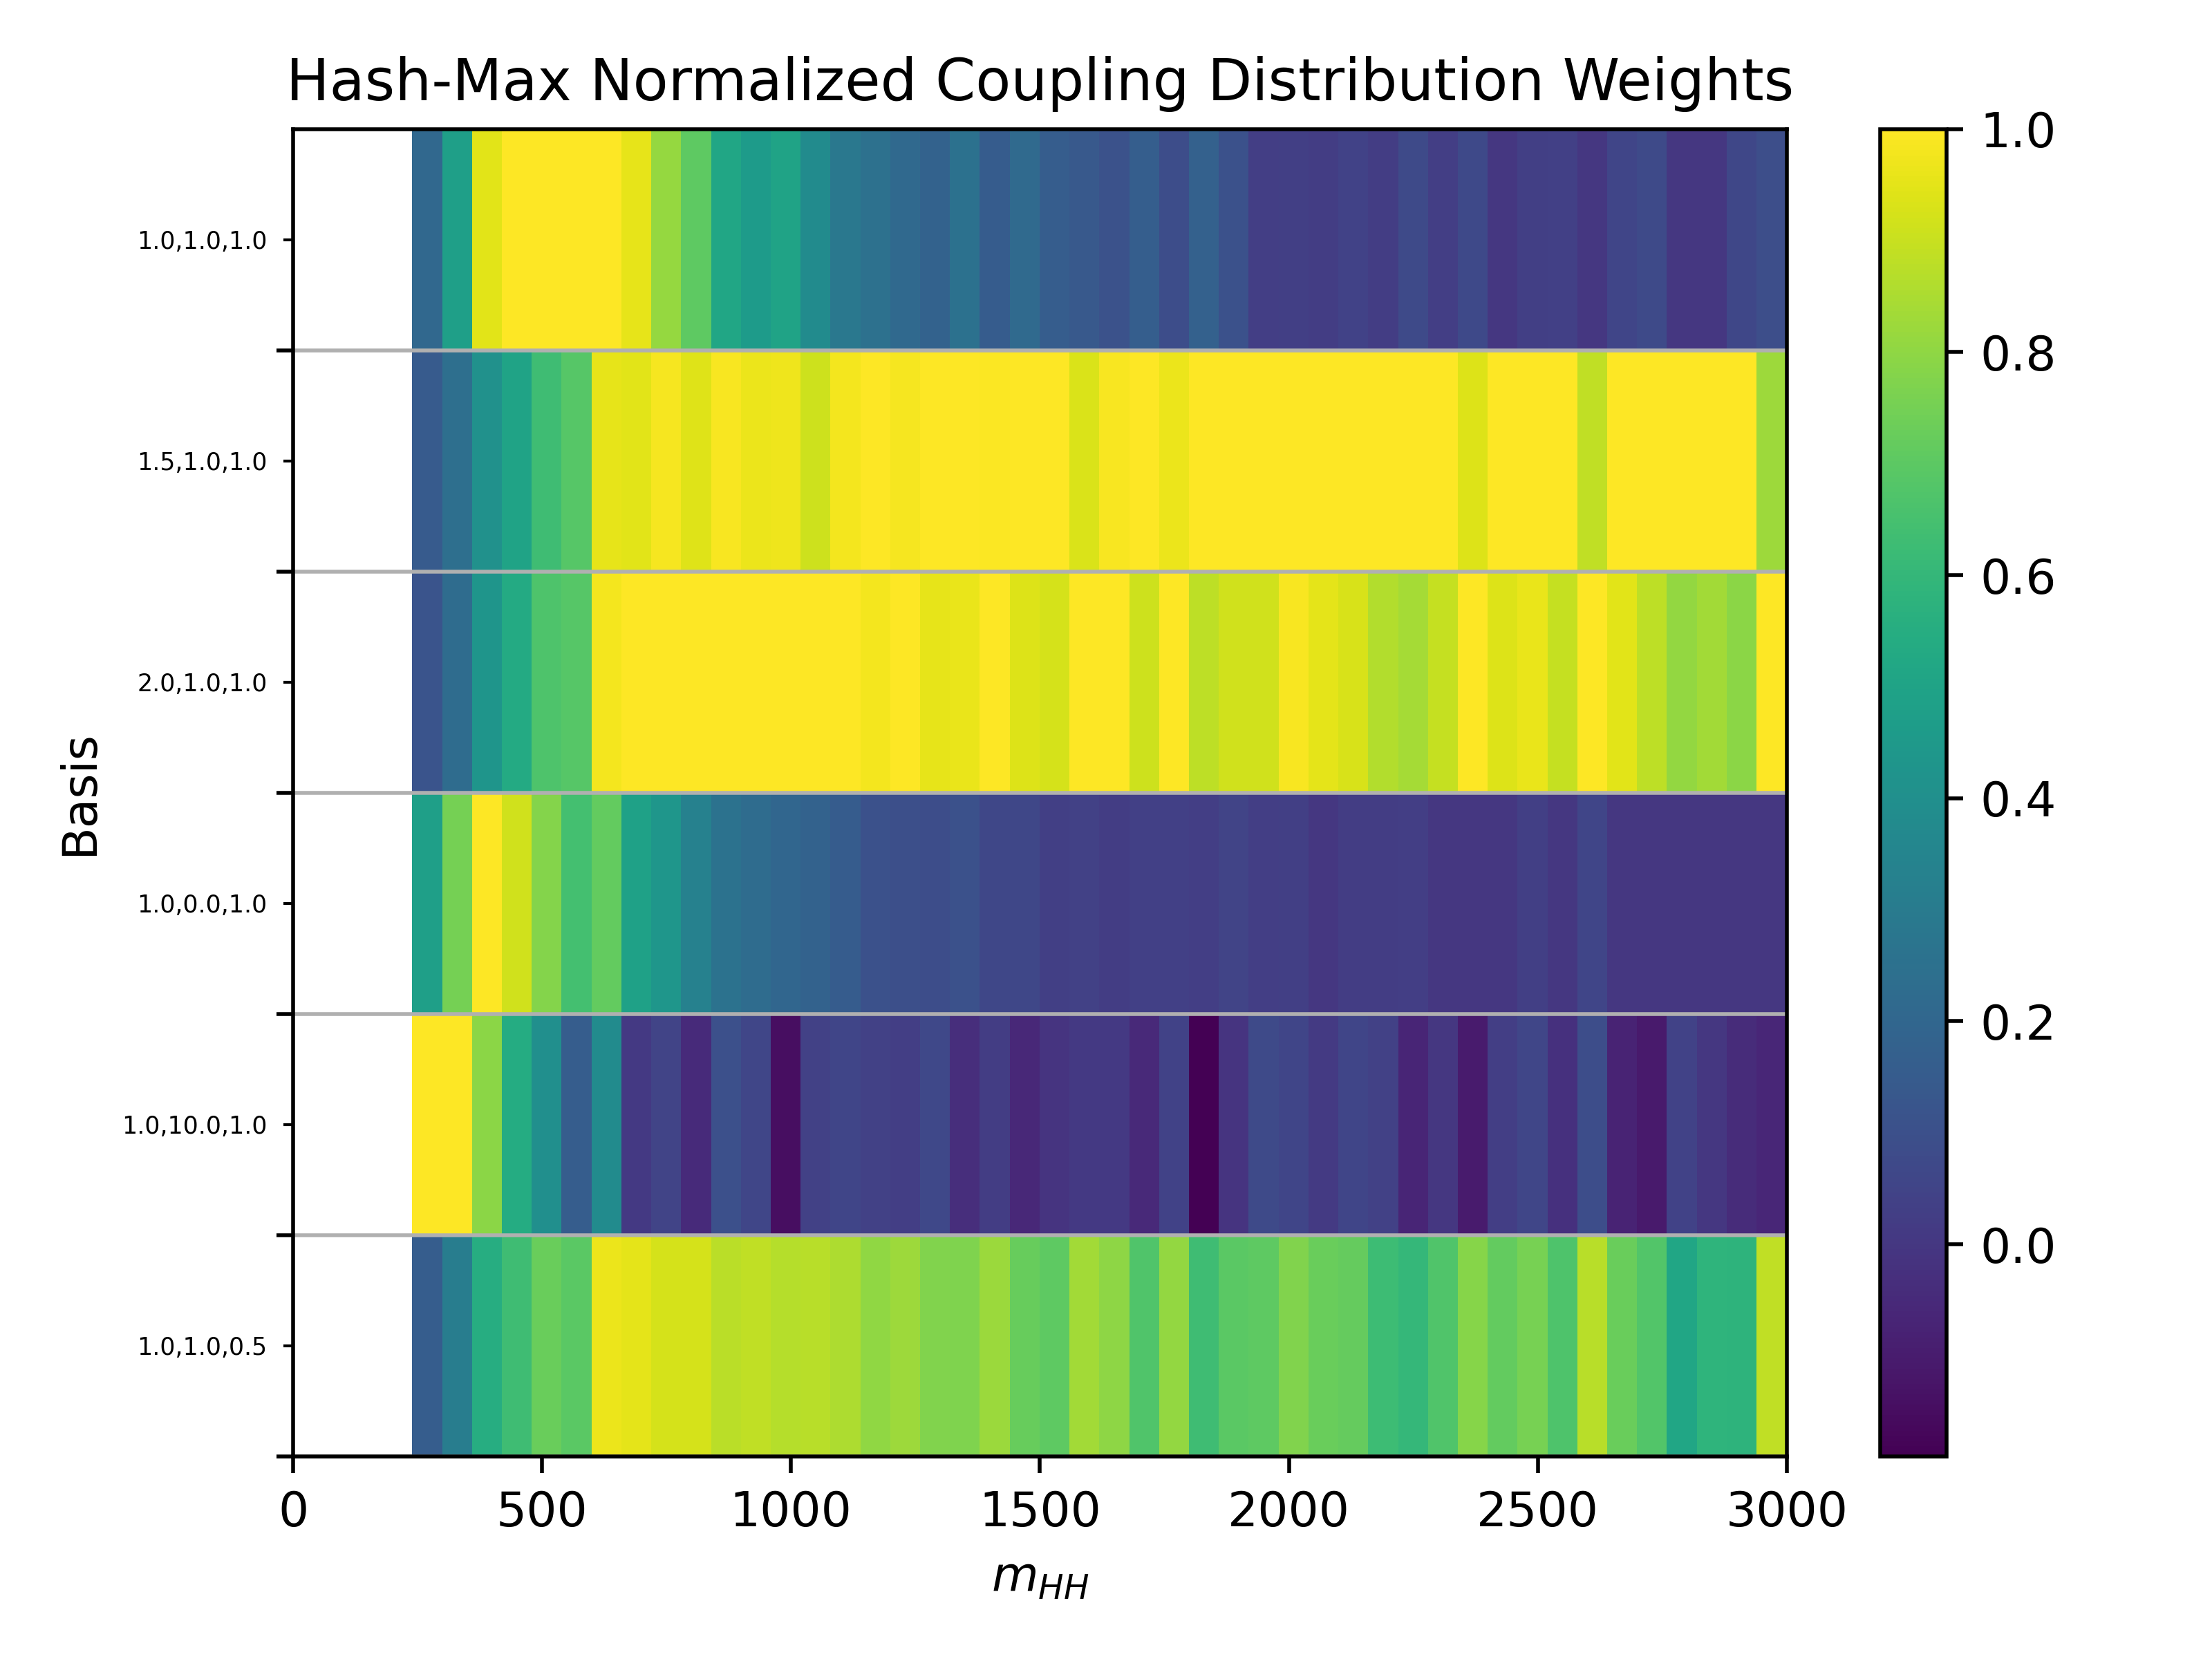
\includegraphics[width=\linewidth,height=\textheight,keepaspectratio]
                {coupling_scan_auto_chosenR0_hash_max}
            \end{figure}

            \end{center}
        \end{column}
        \begin{column}{0.33\textwidth}
            \begin{center} 
            \resizebox{0.3\textheight}{!}{\begin{tabular}{ |l|l|l| }
                \hline
                \textbf {$\kappa_{2V}$} & \textbf {$\kappa_\lambda$} & \textbf {$\kappa_V$} \\
                \hline
                 1.  &  1. &  1.  \\
                 1.5 &  1. &  1.  \\
                 2.  &  1. &  1.  \\
                 1.  &  0. &  1.  \\
                 1.  & 10. &  1.  \\
                 1.  &  1. &  1.5 \\
                \hline
            \end{tabular}}

            \begin{figure}
                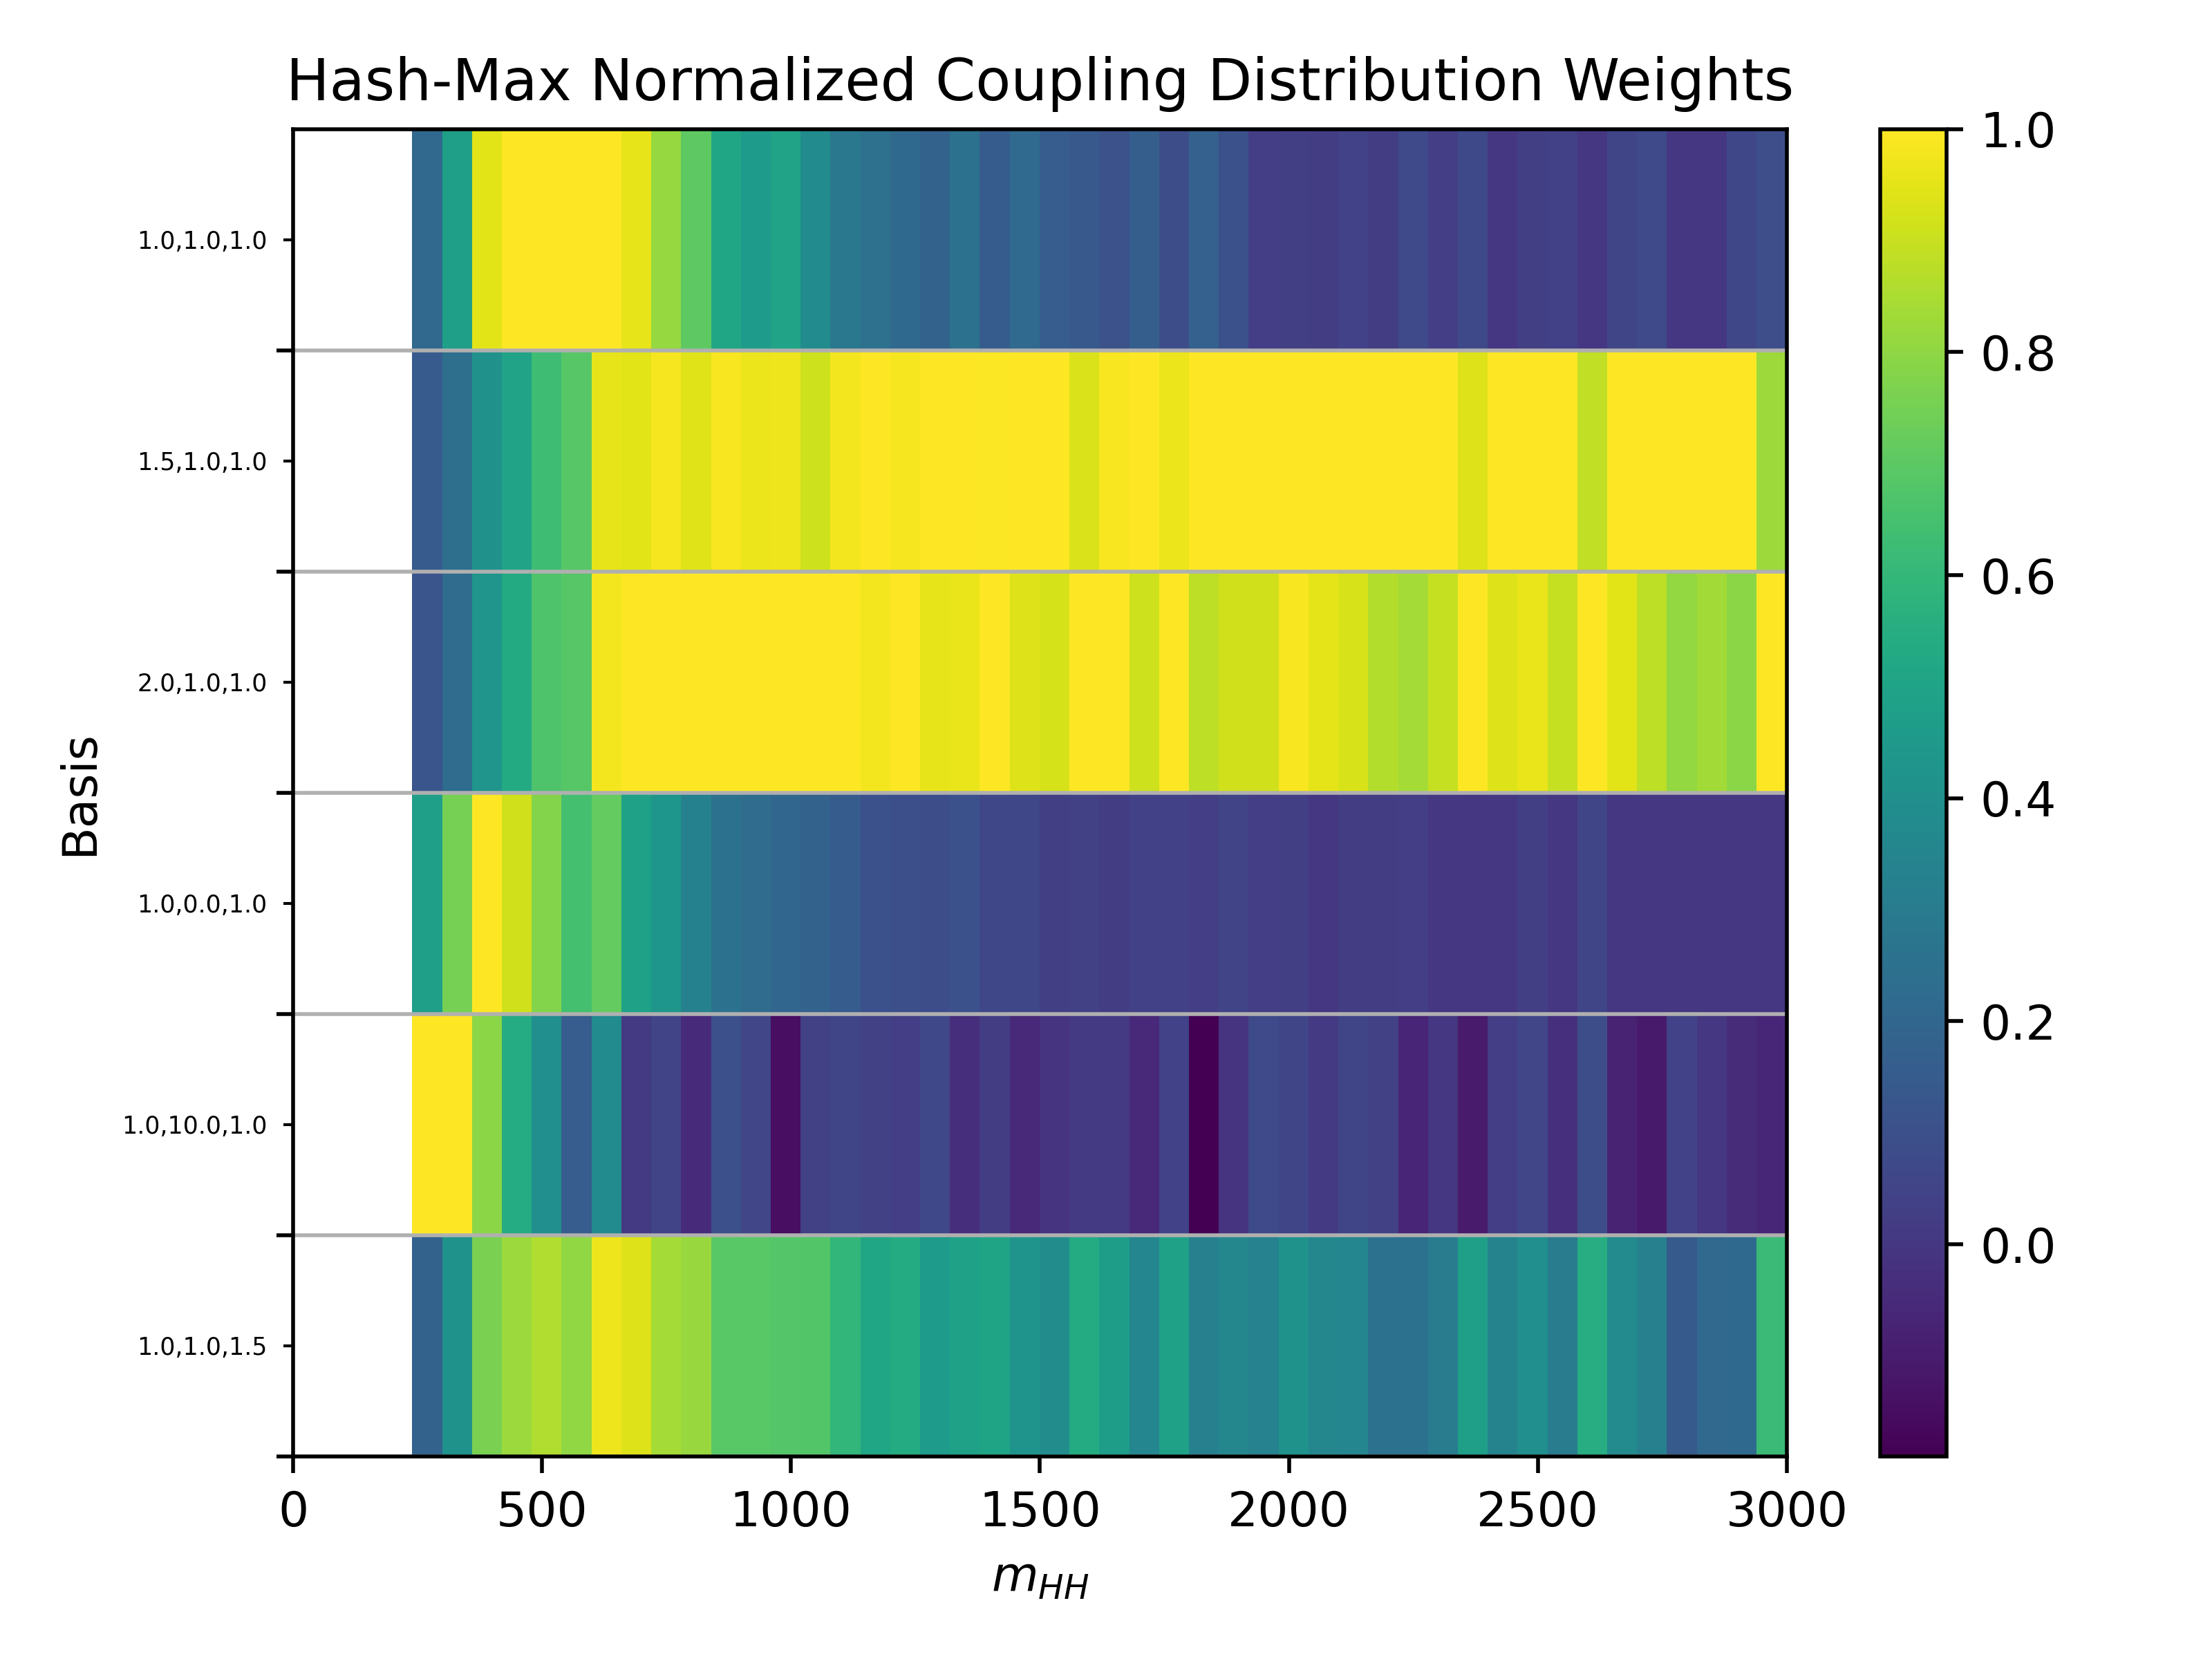
\includegraphics[width=\linewidth,height=\textheight,keepaspectratio]
                {coupling_scan_auto_chosenR1_hash_max}
            \end{figure}

            \end{center}
        \end{column}
        \begin{column}{0.33\textwidth}
            \begin{center} 
            \resizebox{0.3\textheight}{!}{\begin{tabular}{ |l|l|l| }
                \hline
                \textbf {$\kappa_{2V}$} & \textbf {$\kappa_\lambda$} & \textbf {$\kappa_V$} \\
                \hline
                 1.  &  1. &  1.  \\
                 1.5 &  1. &  1.  \\
                 2.  &  1. &  1.  \\
                 1.  &  0. &  1.  \\
                 1.  & 10. &  1.  \\
                 0.  &  0. &  1.  \\
                \hline
            \end{tabular}}

            \begin{figure}
                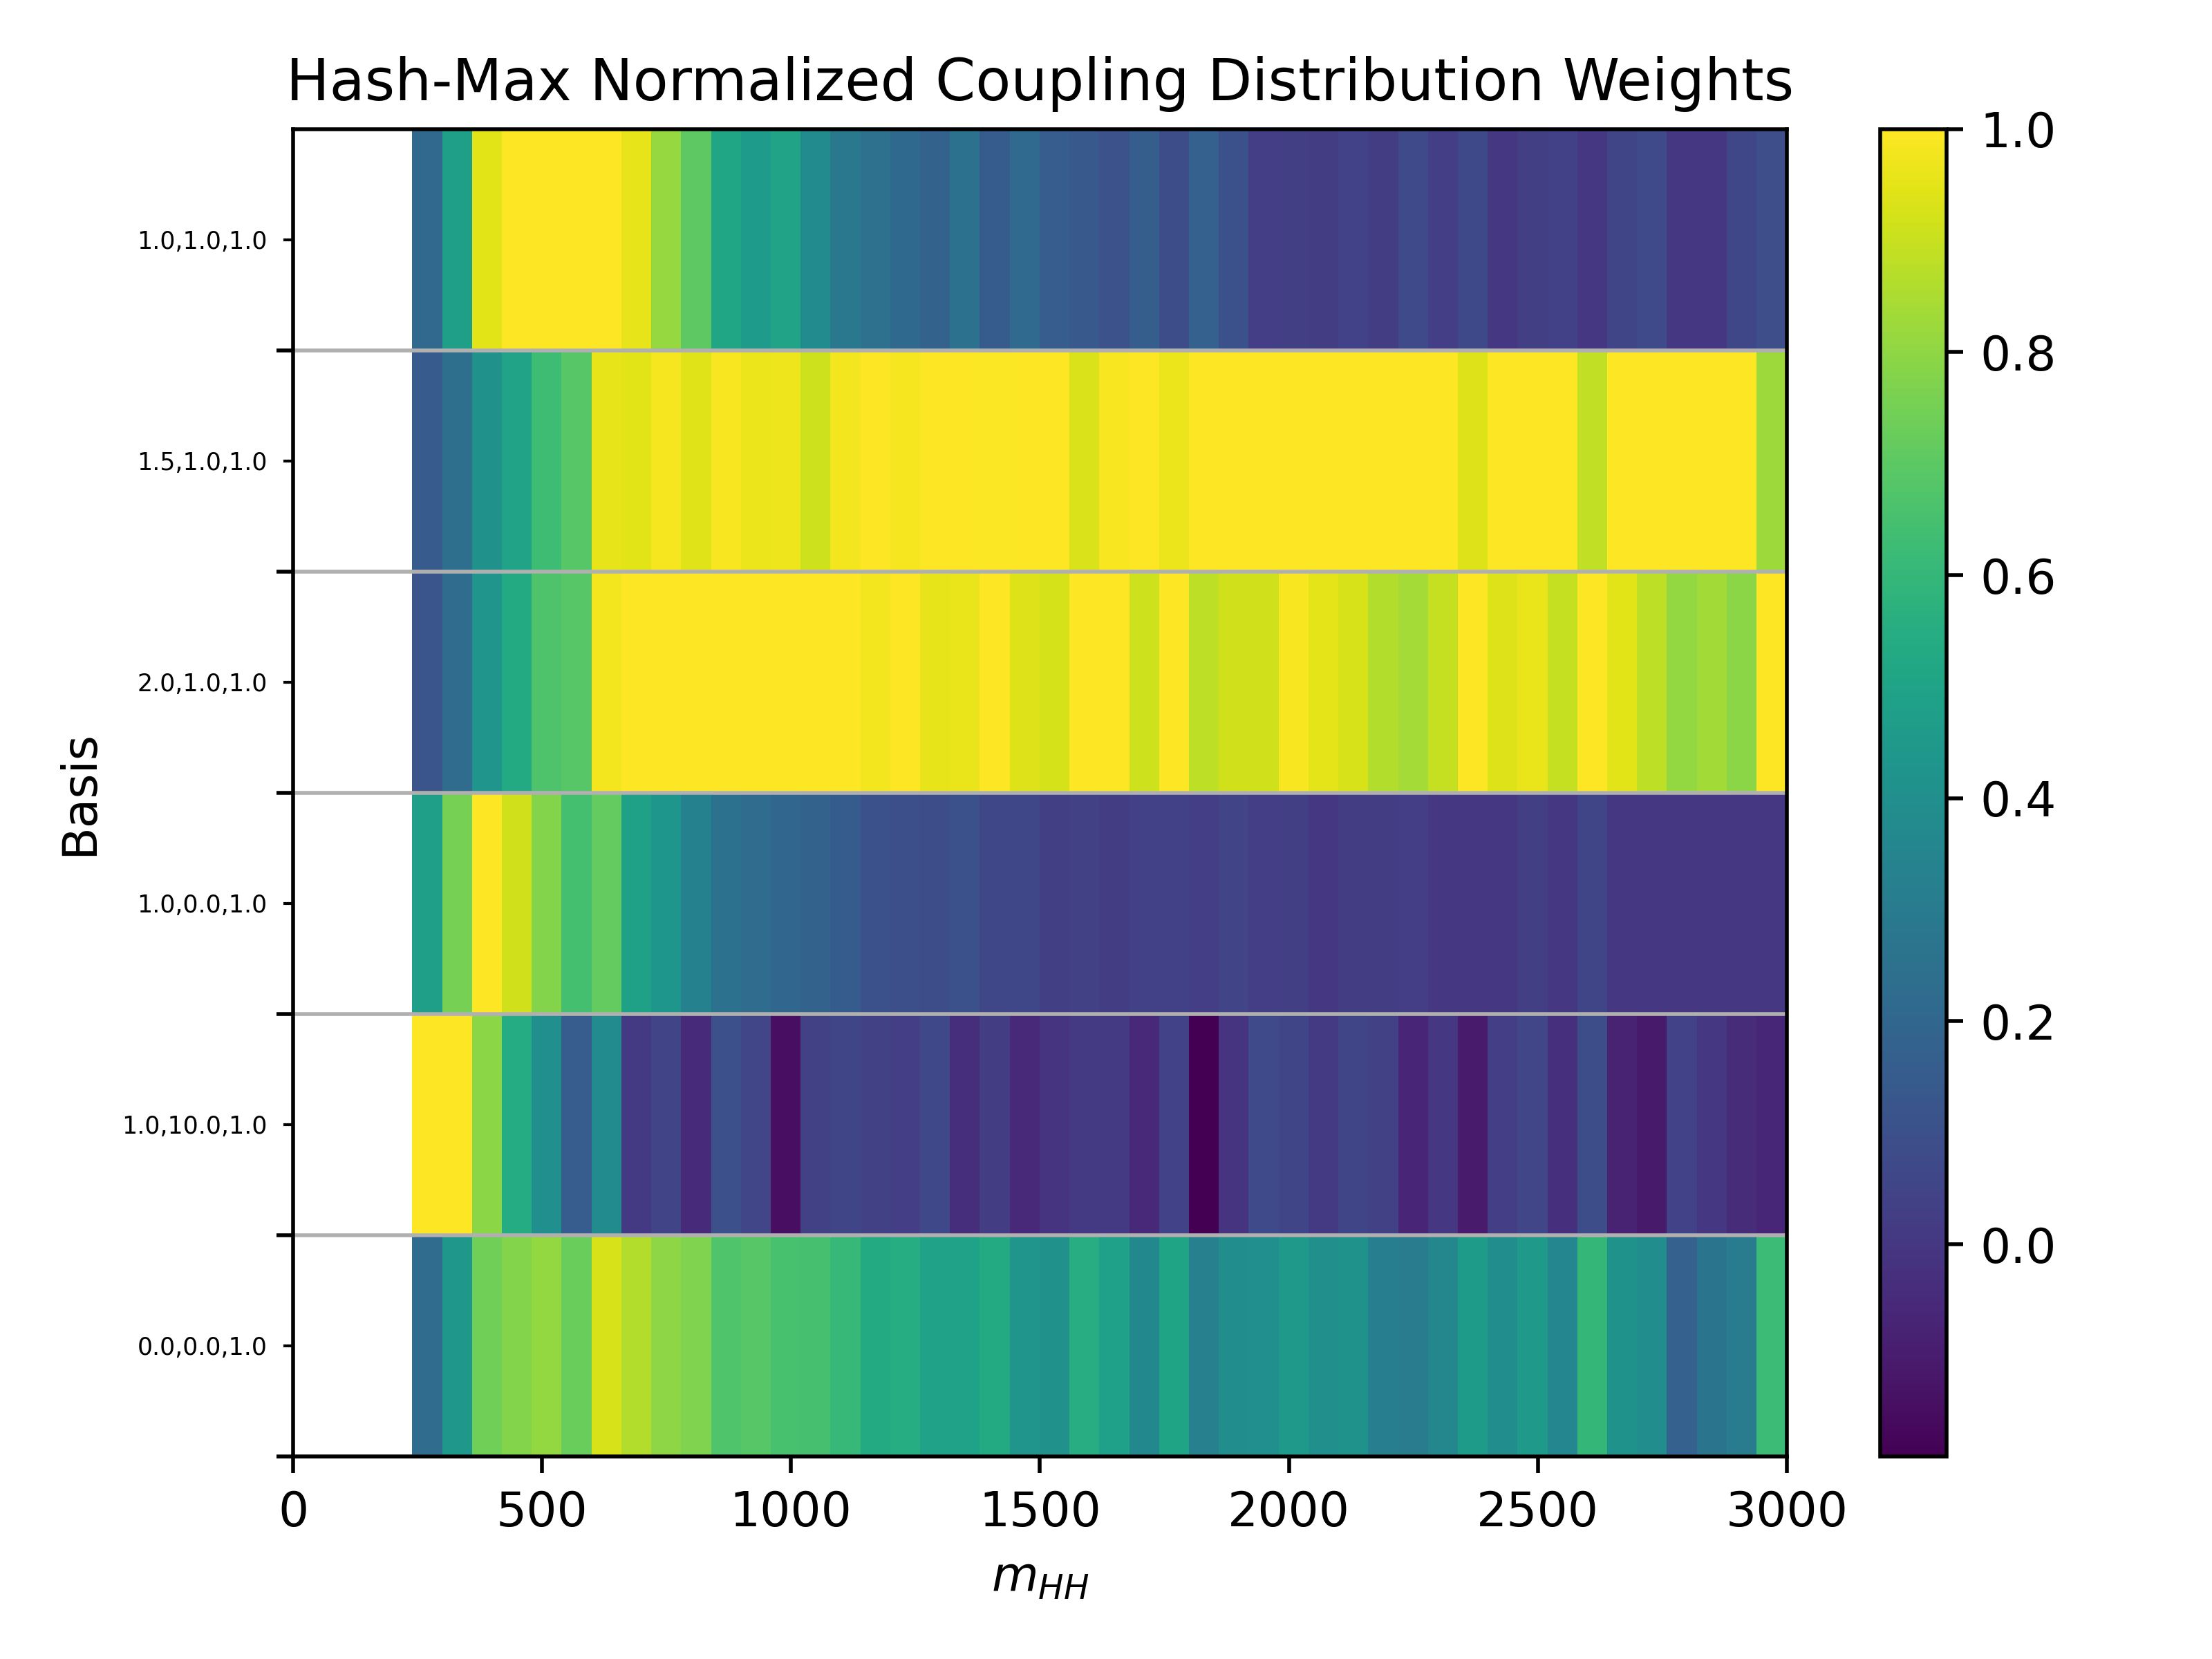
\includegraphics[width=\linewidth,height=\textheight,keepaspectratio]
                {coupling_scan_auto_chosenR2_hash_max}
            \end{figure}

            \end{center}
        \end{column}
    \end{columns}
}

    \section{Orthogonal Basis States}

\frame{
    \frametitle{$M_{HH}$ Truth Reweighting}
    Use the six truth basis samples to reweight individual SM (Truth) events, 
    based on $m_{HH}$ of event, via reweight function:

    \vspace{5mm}

    $ w(\kvv=x,\kl=y,\kv=z, \textrm{bin}\,i) 
     = \frac{m_{HH}^{\kvv=x,\kl=y,\kv=z,i} }{ m_{HH}^{\kvv=1,\kl=1,\kv=1,i}}$

}

\displayfour{Comparing Reweighted Distributions with Linear Combination and Generated Sample}
{truth_rwgt_DUAL_HH_m_cvv0p5cl1p0cv1p0}
{truth_rwgt_DUAL_HH_m_cvv1p0cl2p0cv1p0}
{truth_rwgt_DUAL_HH_m_cvv0p0cl1p0cv1p0}
{truth_rwgt_DUAL_HH_m_cvv3p0cl1p0cv1p0}

    \announcesection{Reweighting Other Distributions}

\displayfour{Di-Higgs $\Delta \eta$}
{truth_rwgt_HH_eta_cvv0p5cl1p0cv1p0}
{truth_rwgt_HH_eta_cvv1p0cl2p0cv1p0}
{truth_rwgt_HH_eta_cvv0p0cl1p0cv1p0}
{truth_rwgt_HH_eta_cvv3p0cl1p0cv1p0}

\displayfour{Di-Higgs $p_T$}
{truth_rwgt_HH_pt_cvv0p5cl1p0cv1p0}
{truth_rwgt_HH_pt_cvv1p0cl2p0cv1p0}
{truth_rwgt_HH_pt_cvv0p0cl1p0cv1p0}
{truth_rwgt_HH_pt_cvv3p0cl1p0cv1p0}

\displayfour{Initial Scatter Jet Invariant Mass}
{truth_rwgt_jj_M_cvv0p5cl1p0cv1p0}
{truth_rwgt_jj_M_cvv1p0cl2p0cv1p0}
{truth_rwgt_jj_M_cvv0p0cl1p0cv1p0}
{truth_rwgt_jj_M_cvv3p0cl1p0cv1p0}

\displayfour{Initial Scatter Jet $\Delta \eta$}
{truth_rwgt_jj_eta_cvv0p5cl1p0cv1p0}
{truth_rwgt_jj_eta_cvv1p0cl2p0cv1p0}
{truth_rwgt_jj_eta_cvv0p0cl1p0cv1p0}
{truth_rwgt_jj_eta_cvv3p0cl1p0cv1p0}

\displayfour{Initial Scatter Jet $p_T$}
{truth_rwgt_jj_pt_cvv0p5cl1p0cv1p0}
{truth_rwgt_jj_pt_cvv1p0cl2p0cv1p0}
{truth_rwgt_jj_pt_cvv0p0cl1p0cv1p0}
{truth_rwgt_jj_pt_cvv3p0cl1p0cv1p0}



    \section{Conclusion}
    \frame{
        \frametitle{Conclusions}
        \begin{itemize} {
            {\large \item Linear combinations are able to effectively reweight distributions at truth level}
            {\large \item There are still significant problems with using truth distributions to reweight reconstructed events though}
            {\large \item Investigation still ongoing, with further details expected by the next meeting}
            {\large \item These issues are unfortunately delaying completion of the VBF reweighting tool}
        } \end{itemize}
    }

    %\announcesection{Backup}

\end{document}
